\documentclass[12pt, oneside]{article}
\usepackage[letterpaper, margin=1in, headsep=0.5in]{geometry}
\usepackage[english]{babel}
\usepackage[utf8]{inputenc}
\usepackage{amsmath}
\usepackage{amsfonts}
\usepackage{amssymb}
\usepackage{tikz}
\usetikzlibrary{quotes, angles}
\usepackage{graphicx}
%\usepackage{pgfplots}
%\pgfplotsset{width=10cm,compat=1.9}
%\usepgfplotslibrary{statistics}
%\usepackage{pgfplotstable}
%\usepackage{tkz-fct}
%\usepackage{venndiagram}

\usepackage{fancyhdr}
\pagestyle{fancy}
\fancyhf{}
\rhead{\thepage \\Name: \hspace{1.5in}.\\}
\lhead{BECA / Dr. Huson / Geometry 10th Grade\\* Unit 1: Introduction to Geometry}

\renewcommand{\headrulewidth}{0pt}

\begin{document}
\subsubsection*{Quiz Corrections 1.4: Correct Friday's Do Now Quiz, complete this review, and staple them together. Due tomorrow for one-half of your missed points.}
  \vspace{0.5cm}
  \begin{enumerate}
    \item The points where a line segment begins and ends are the $\rule{4cm}{0.15mm}$. \smallskip
    \item A(n) $\rule{4cm}{0.15mm}$ is a portion of a line that includes two points and all of the collinear points between the two points.\smallskip
    \item A(n) $\rule{4cm}{0.15mm}$ is a portion of a line that begins with a single point and extends infinitely in one direction.
    \item Points that are all located on the same line are $\rule{4cm}{0.15mm}$.\bigskip
    \item Two or more line segments of equal measure are $\rule{4cm}{0.15mm}$.\bigskip
    \item A flat surface is a(n) $\rule{4cm}{0.15mm}$. \bigskip
    \item A(n) $\rule{4cm}{0.15mm}$ is a straight continuous arrangement of an infinite number of points.

  \item Use symbols to write the name of each geometric figure.
  \begin{enumerate}
  \item %Ray DE
    \begin{tikzpicture}
      \draw [->, thick] (0,0)--(3,1.5);
      \draw [fill] (0,0) circle [radius=0.05] node[below]{$D$};
      \draw [fill] (2,1) circle [radius=0.05] node[below]{$E$};
    \end{tikzpicture} \bigskip
  \item \hspace{1cm}%Line AB
    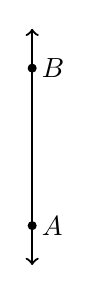
\begin{tikzpicture}
      \draw [<->, thick] (1,0)--(1,3);
      \draw [fill] (1,0.5) circle [radius=0.05] node[right]{$A$};
      \draw [fill] (1,2.5) circle [radius=0.05] node[right]{$B$};
    \end{tikzpicture} \bigskip
    \item %Line segment XY
      \begin{tikzpicture}
        \draw [-, thick] (1,0)--(0,2);
        \draw [fill] (1,0) circle [radius=0.05] node[below]{$X$};
        \draw [fill] (0,2) circle [radius=0.05] node[left]{$Y$};
      \end{tikzpicture}
  \end{enumerate}
  \end{enumerate}

\newpage
\subsubsection*{Do Now 1.4: Notation and terminology} % DONE
  \begin{enumerate}
    \item I have a compass, ruler, protractor, notebook, and folder (circle one). Yes \qquad No

    \item Use each term according to its geometric meaning: ``sketch", ``draw", ``construct".
    \begin{enumerate}
      \item $\rule{4cm}{0.15mm}$ is to make a freehand diagram showing important features. \smallskip
      \item $\rule{4cm}{0.15mm}$ is to depict with accurate measures using ruler, protractor, and compass. \smallskip
      \item $\rule{4cm}{0.15mm}$ is a formal, logical process to create geometric figures using only a straightedge and compass.
    \end{enumerate} \smallskip

  \item Two or more line segments of equal measure are $\rule{4cm}{0.15mm}$.
    \bigskip
  \item Given $\overline{ABC}$, $AB=10$, and $BC=4$.
  \begin{enumerate}
    \item Find ${AC}$.\\[0.75cm]
      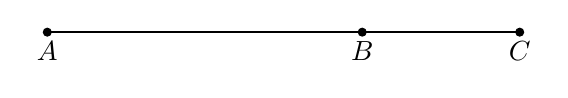
\begin{tikzpicture}
        \draw [-, thick] (1,0)--(7,0);
        \draw [fill] (1,0) circle [radius=0.05] node[below]{$A$};
        \draw [fill] (5,0) circle [radius=0.05] node[below]{$B$};
        \draw [fill] (7,0) circle [radius=0.05] node[below]{$C$};
      \end{tikzpicture} \smallskip
    \item The postulate used in this problem is the \rule{6cm}{0.15mm}.
  \end{enumerate}
  \smallskip

  \item Given $\triangle ABC$ with $\overline{AC} \cong \overline{BC}$. On the diagram mark the congruent line segments with tick marks.
  \begin{center}
  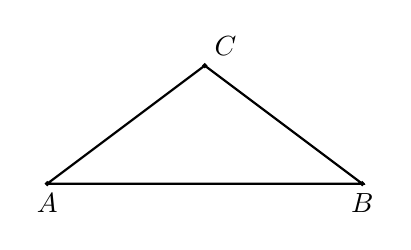
\begin{tikzpicture}[scale=0.5]
    \draw [thick](0,0)--(8,0)--(4,3)--(0,0);
    \draw [fill] (0,0) circle [radius=0.05] node[below]{$A$};
    \draw [fill] (8,0) circle [radius=0.05] node[below]{$B$};
    \draw [fill] (4,3) circle [radius=0.05] node[above right]{$C$};
  \end{tikzpicture}
  \end{center}

  \item Given line segment $\overline{AB}$ with midpoint $M$, that is, $\overline{AM} \cong \overline{BM}$. $AM=2$ cm. Find the length of $\overline{AB}$.\\[0.75cm]
  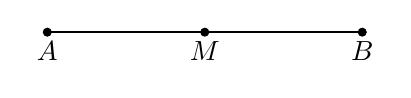
\begin{tikzpicture}
    \draw [-, thick] (1,0)--(5,0);
    \draw [fill] (1,0) circle [radius=0.05] node[below]{$A$};
    \draw [fill] (5,0) circle [radius=0.05] node[below]{$B$};
    \draw [fill] (3,0) circle [radius=0.05] node[below]{$M$};
  \end{tikzpicture}
  \vspace{1cm}

  \item Points that are all located on the same line are $\rule{4cm}{0.15mm}$.
  \item Find the value of $|8.5-3|$.

  \newpage
  \item Given the points $X$ and $Y$, draw $\overrightarrow{YX}$.\\
  \vspace{1cm}
  \begin{center}
    \begin{tikzpicture}
    \draw [fill] (0,2) circle [radius=0.05] node[below]{$X$};
    \draw [fill] (5,0) circle [radius=0.05] node[below]{$Y$};
  \end{tikzpicture}
  \end{center}
  %\vspace{2cm}

  \item Given $\triangle ABC$ write down two congruent line segments using proper notation.\\
  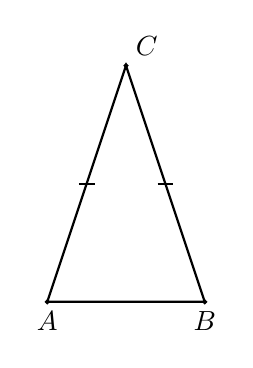
\begin{tikzpicture}[scale=0.5]
    \draw [thick](0,0)--(4,0)--(2,6)--(0,0);
    \draw [fill] (0,0) circle [radius=0.05] node[below]{$A$};
    \draw [fill] (4,0) circle [radius=0.05] node[below]{$B$};
    \draw [fill] (2,6) circle [radius=0.05] node[above right]{$C$};
    \draw [thick] (0.8,3)--(1.2,3); %tick mark
    \draw [thick] (2.8,3)--(3.2,3); %tick mark
  \end{tikzpicture}

  \item Given $\overrightarrow{DE}$, construct circle $E$ with radius $DE$.
  \vspace{4cm}
  \begin{center}
  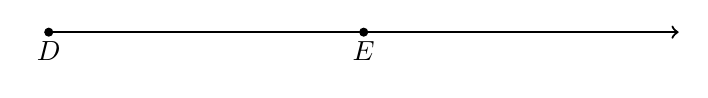
\begin{tikzpicture}
    \draw [->, thick] (0,0)--(8,0);
    \draw [fill] (0,0) circle [radius=0.05] node[below]{$D$};
    \draw [fill] (4,0) circle [radius=0.05] node[below]{$E$};
  \end{tikzpicture}
  \end{center}
  \vspace{4cm}
  Spicy: Complete the construction of an equilateral triangle with one side $\overline{DE}$.
  \end{enumerate}

\newpage
\subsubsection*{Homework 1.4: Geometric diagrams} %DONE
  \begin{enumerate}
    \item A flat surface is a(n) $\rule{4cm}{0.15mm}$.
    \item Use symbols to write the name of the given figure.
      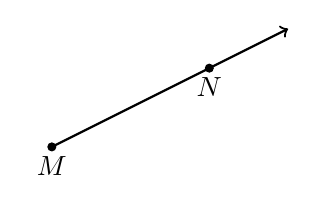
\begin{tikzpicture}
        \draw [->, thick] (0,0)--(3,1.5);
        \draw [fill] (0,0) circle [radius=0.05] node[below]{$M$};
        \draw [fill] (2,1) circle [radius=0.05] node[below]{$N$};
      \end{tikzpicture} \bigskip

    \item Given $\overline{ABC}$, $AB=2x+1$, $BC=x-1$, and $AC=9$. Find ${AB}$.\\[0.5in]
        %\vspace{1cm}
       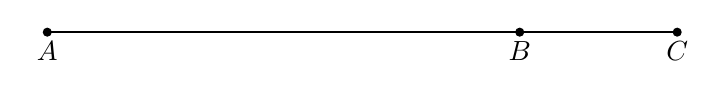
\begin{tikzpicture}
        \draw [-, thick] (-1,0)--(7,0);
        \draw [fill] (-1,0) circle [radius=0.05] node[below]{$A$};
        \draw [fill] (5,0) circle [radius=0.05] node[below]{$B$};
        \draw [fill] (7,0) circle [radius=0.05] node[below]{$C$};
      \end{tikzpicture} \vspace{4cm}

    \item Write down the name of two line segments shown in the diagram below using proper geometric notation.
    \begin{center}
    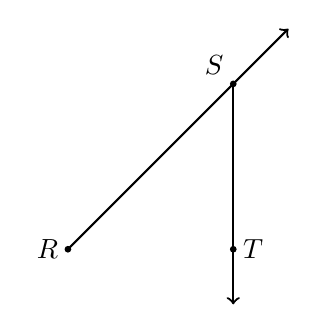
\begin{tikzpicture}[scale=0.7]
      \draw [->, thick] (0,0)--(4,4);
      \draw [->, thick] (3,3)--(3,-1);
      \draw [fill] (0,0) circle [radius=0.05] node[left]{$R$};
      \draw [fill] (3,3) circle [radius=0.05] node[above left]{$S$};
      \draw [fill] (3,0) circle [radius=0.05] node[right]{$T$};
    \end{tikzpicture}
    \end{center}


    \item Identify two lines in the given plane.\\[0.25in]
      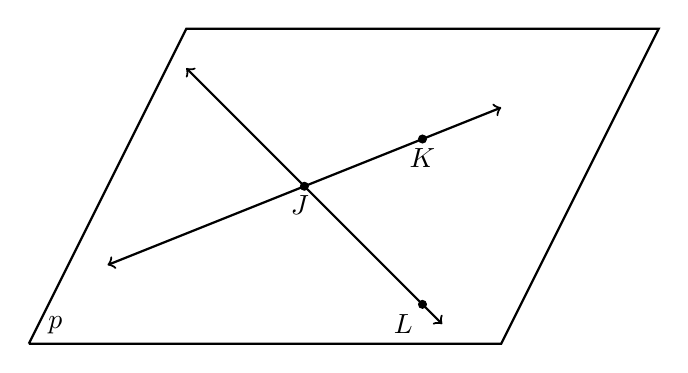
\begin{tikzpicture}
        \draw [thick](0,0) node[above right]{$\ p$} --(6,0)--(8,4)--(2,4)--(0,0);
        \draw [<->, thick] (1,1)--(6,3);
        \draw [fill] (3.5,2) circle [radius=0.05] node[below]{$J \ $};
        \draw [fill] (5,2.6) circle [radius=0.05] node[below]{$K$};
        \draw [<->, thick] (2,3.5)--(5.25,.25);
        \draw [fill] (5,0.5) circle [radius=0.05] node[below left]{$L$};
      \end{tikzpicture} %\vspace{2cm}

    \newpage
    \item Given $\triangle ABC$ with $\overline{AC} \cong \overline{BC}$. $AC=x+7$ and $BC=2x+1$. Find $AC$.\\[0.5cm]
    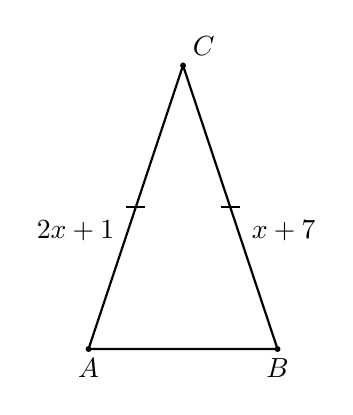
\begin{tikzpicture}[scale=0.6]
      \draw [thick](0,0)--(4,0)--(2,6)--(0,0);
      \draw [fill] (0,0) circle [radius=0.05] node[below]{$A$};
      \draw [fill] (4,0) circle [radius=0.05] node[below]{$B$};
      \draw [fill] (2,6) circle [radius=0.05] node[above right]{$C$};
      \draw [thick] (0.8,3)--(1.2,3); %tick mark
      \draw [thick] (2.8,3)--(3.2,3); %tick mark
      \node [right] at (3.25,2.5){$x+7$};
      \node [left] at (0.75,2.5){$2x+1$};
    \end{tikzpicture}

    \item $\rule{4cm}{0.15mm}$ is to make a freehand diagram showing important features. \smallskip

    \item Given $A(4,3)$ and $B(6,4)$. What is the slope of $\overleftrightarrow{AB}$? Use the formula $\displaystyle m=\frac{y_2-y_1}{x_2-x_1}$. \vspace{4cm}

    \item Points that are all located on the same line are $\rule{4cm}{0.15mm}$.\bigskip


  \item Spicy: Given the rectangle $ABCD$ with $\overline{AB} \cong \overline{CD}$ and $\overline{BC} \cong \overline{DA}$. $AB=x+7$ and $\displaystyle CD=\frac{4x+2}{2}$. Find $AB$.\\[0.5cm]
  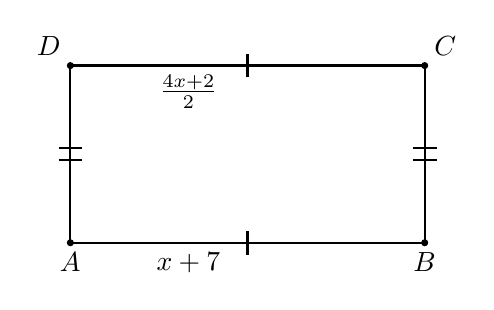
\begin{tikzpicture}[scale=0.75]
    \draw [thick](0,0)--(6,0)--(6,3)--(0,3)--(0,0);
    \draw [fill] (0,0) circle [radius=0.05] node[below]{$A$};
    \draw [fill] (6,0) circle [radius=0.05] node[below]{$B$};
    \draw [fill] (6,3) circle [radius=0.05] node[above right]{$C$};
    \draw [fill] (0,3) circle [radius=0.05] node[above left]{$D$};
    \draw [thick] (3,-0.2)--(3,0.2); %tick mark
    \draw [thick] (3,2.8)--(3,3.2); %tick mark
    \draw [thick] (-0.2,1.4)--(0.2,1.4); %tick mark
    \draw [thick] (-0.2,1.6)--(0.2,1.6); %tick mark
    \draw [thick] (5.8,1.4)--(6.2,1.4); %tick mark
    \draw [thick] (5.8,1.6)--(6.2,1.6); %tick mark
    \node [below] at (2,0){$x+7$};
    \node [below] at (2,3){$\frac{4x+2}{2}$};
  \end{tikzpicture}
  %\vspace{4cm}

  \end{enumerate}

\newpage
\subsubsection*{Do Now 1.5: Plane geometry, measure lengths}
  \begin{enumerate}
    \item Accurately measure the length of each side of $\triangle ABC$ in centimeters (cm) to the nearest tenth.
      \bigskip
    \begin{enumerate}
      \item $AB=\rule{2cm}{0.15mm}$ \bigskip
      \item $BC=\rule{2cm}{0.15mm}$ \bigskip
      \item $AC=\rule{2cm}{0.15mm}$
    \end{enumerate}
    \begin{center}
    \begin{tikzpicture}%[scale=0.5]
      \draw [thick](0,0)--(8,1)--(2,4)--(0,0);
      \draw [fill] (0,0) circle [radius=0.05] node[below]{$A$};
      \draw [fill] (8,1) circle [radius=0.05] node[below]{$B$};
      \draw [fill] (2,4) circle [radius=0.05] node[above right]{$C$};
    \end{tikzpicture}
    \end{center}

  \item Draw a figure for each description. Draw the line or segment and label all points mentioned in the description.
  \begin{enumerate}
    \item The line segment $XY$ such that the distance between points $X$ and $Y$ is 6 cm. \vspace{2cm}
    \item Points $A$, $D$, and $X$ are collinear such that point $A$ is located halfway between points $D$ and $X$. (hint: mark the congruent segments with tick marks) \vspace{2cm}
    \item Points $A$, $B$, and $C$ are collinear such that point $B$ is between points $A$ and $C$ and the distance between points $A$ and $B$ is twice the distance between points $B$ and $C$. \vspace{2cm}
  \end{enumerate}



  \end{enumerate}

\newpage
\subsubsection*{Homework 1.5: Segment addition. Reminder construction project due tomorrow}
  \begin{enumerate}
    \item Given $\overline{ABC}$, $AB=4x-9$, $BC=x+11$, $AC=22$. Find ${AB}$. Show each step:\\[0.5in]
    \begin{center}
      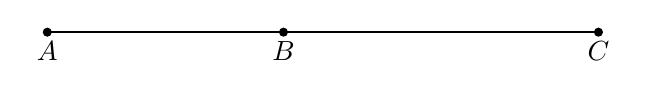
\begin{tikzpicture}
         \draw [-, thick] (0,0)--(7,0);
         \draw [fill] (0,0) circle [radius=0.05] node[below]{$A$};
         \draw [fill] (3,0) circle [radius=0.05] node[below]{$B$};
         \draw [fill] (7,0) circle [radius=0.05] node[below]{$C$};
      \end{tikzpicture}
    \end{center}
      \vspace{1cm}
    \begin{enumerate}
      \item Sketch and label the situation
      \item Write a geometric equation\\
      \begin{flushright} Segment addition\\ postulate \end{flushright}
      \item Substitute algebraic values
      \item Solve for the unknown \vspace{3cm}
      \begin{center} $x=$ \rule{1cm}{0.15} \end{center}
      \item Answer the question\\
      \begin{center} $AB=$ \rule{1cm}{0.15} \end{center}
      \item Check your answer
    \end{enumerate}


    %\item Segment Addition Puzzle (add vocab \& algebra, abs value, review)
  \end{enumerate}

\newpage
\subsubsection*{Do Now Quiz 1.6: notation, segment addition algebra} %duplicate of 1.4 Homework
\begin{enumerate}
  \item A flat surface is a(n) $\rule{4cm}{0.15mm}$.
  \item Use symbols to write the name of the given figure.
    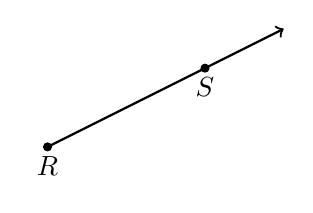
\begin{tikzpicture}
      \draw [->, thick] (0,0)--(3,1.5);
      \draw [fill] (0,0) circle [radius=0.05] node[below]{$R$};
      \draw [fill] (2,1) circle [radius=0.05] node[below]{$S$};
    \end{tikzpicture} \bigskip

  \item Given $\overline{ABC}$, $AB=2x+1$, $BC=x-1$, and $AC=9$. Find ${AB}$.\\[0.5in]
      %\vspace{1cm}
     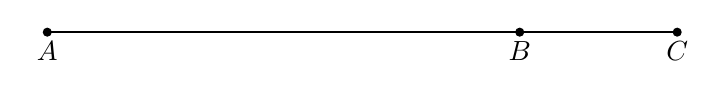
\begin{tikzpicture}
      \draw [-, thick] (-1,0)--(7,0);
      \draw [fill] (-1,0) circle [radius=0.05] node[below]{$A$};
      \draw [fill] (5,0) circle [radius=0.05] node[below]{$B$};
      \draw [fill] (7,0) circle [radius=0.05] node[below]{$C$};
    \end{tikzpicture} \vspace{2cm}

  \item Write down the name of two line segments shown in the diagram below using proper geometric notation.
  \begin{center}
  \begin{tikzpicture}
    \draw [->, thick] (0,0)--(4,4);
    \draw [->, thick] (3,3)--(3,-1);
    \draw [fill] (0,0) circle [radius=0.05] node[left]{$R$};
    \draw [fill] (3,3) circle [radius=0.05] node[above left]{$S$};
    \draw [fill] (3,0) circle [radius=0.05] node[right]{$T$};
  \end{tikzpicture}
  \end{center}

  \item Identify two lines in the given plane.\\[0.25in]
    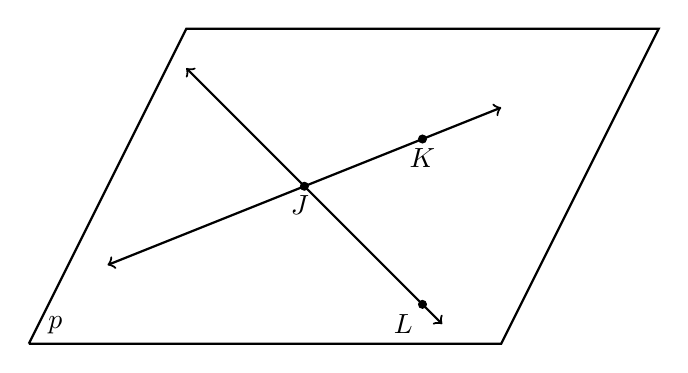
\begin{tikzpicture}
      \draw [thick](0,0) node[above right]{$\ p$} --(6,0)--(8,4)--(2,4)--(0,0);
      \draw [<->, thick] (1,1)--(6,3);
      \draw [fill] (3.5,2) circle [radius=0.05] node[below]{$J \ $};
      \draw [fill] (5,2.6) circle [radius=0.05] node[below]{$K$};
      \draw [<->, thick] (2,3.5)--(5.25,.25);
      \draw [fill] (5,0.5) circle [radius=0.05] node[below left]{$L$};
    \end{tikzpicture} \vspace{2cm}

  \item Given $\triangle ABC$ with $\overline{AC} \cong \overline{BC}$. $AC=x+7$ and $BC=2x+1$. Find $AC$.\\[0.5cm]
  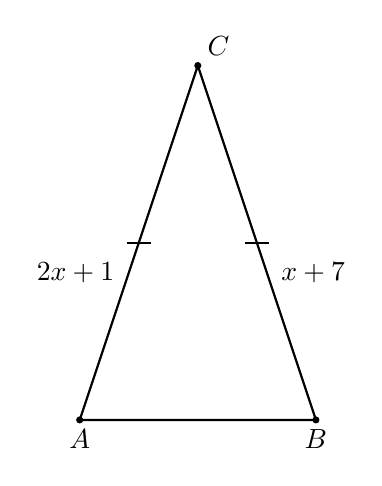
\begin{tikzpicture}[scale=0.75]
    \draw [thick](0,0)--(4,0)--(2,6)--(0,0);
    \draw [fill] (0,0) circle [radius=0.05] node[below]{$A$};
    \draw [fill] (4,0) circle [radius=0.05] node[below]{$B$};
    \draw [fill] (2,6) circle [radius=0.05] node[above right]{$C$};
    \draw [thick] (0.8,3)--(1.2,3); %tick mark
    \draw [thick] (2.8,3)--(3.2,3); %tick mark
    \node [right] at (3.25,2.5){$x+7$};
    \node [left] at (0.75,2.5){$2x+1$};
  \end{tikzpicture}

  \item $\rule{4cm}{0.15mm}$ is to make a freehand diagram showing important features. \smallskip

  \item Given $A(4,3)$ and $B(6,4)$. What is the slope of $\overleftrightarrow{AB}$? Use the formula $\displaystyle m=\frac{y_2-y_1}{x_2-x_1}$. \vspace{3cm}

  \item Points that are all located on the same line are $\rule{4cm}{0.15mm}$.\bigskip

  \item Given the rectangle $ABCD$ with $\overline{AB} \cong \overline{CD}$ and $\overline{BC} \cong \overline{DA}$. $AB=x+7$ and $\displaystyle CD=\frac{4x+2}{2}$. Find $AB$.\\[0.5cm]
  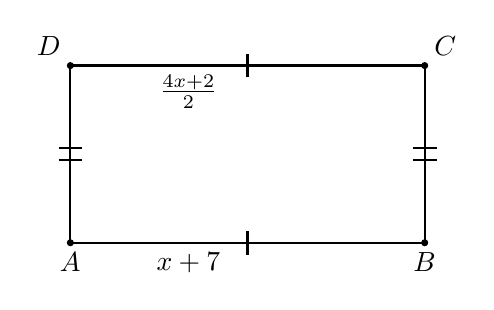
\begin{tikzpicture}[scale=0.75]
    \draw [thick](0,0)--(6,0)--(6,3)--(0,3)--(0,0);
    \draw [fill] (0,0) circle [radius=0.05] node[below]{$A$};
    \draw [fill] (6,0) circle [radius=0.05] node[below]{$B$};
    \draw [fill] (6,3) circle [radius=0.05] node[above right]{$C$};
    \draw [fill] (0,3) circle [radius=0.05] node[above left]{$D$};
    \draw [thick] (3,-0.2)--(3,0.2); %tick mark
    \draw [thick] (3,2.8)--(3,3.2); %tick mark
    \draw [thick] (-0.2,1.4)--(0.2,1.4); %tick mark
    \draw [thick] (-0.2,1.6)--(0.2,1.6); %tick mark
    \draw [thick] (5.8,1.4)--(6.2,1.4); %tick mark
    \draw [thick] (5.8,1.6)--(6.2,1.6); %tick mark
    \node [below] at (2,0){$x+7$};
    \node [below] at (2,3){$\frac{4x+2}{2}$};
  \end{tikzpicture}
  \vspace{4cm}

\end{enumerate}

\newpage
\subsubsection*{Homework 1.6: Angle notation}
  \begin{enumerate}
    \item \tikz \draw (2,0) coordinate (A) -- (0,0) coordinate (B)
             -- (1,1) coordinate (C)
      pic [draw, ->] {angle=A--B--C}; %pic ["$K$"] naming not working


  \end{enumerate}

\newpage
\subsubsection*{Do Now 1.7: Laptop setup}
  \begin{enumerate}
    \item Deltamath
  \end{enumerate}

\newpage
\subsubsection*{Homework 1.7: Angle measurement}
  \begin{enumerate}
  \item \tikz \draw (2,0) coordinate (A) -- (0,0) coordinate (B)
           -- (1,1) coordinate (C)
    pic [draw, ->] {angle=A--B--C}; %pic ["$K$"] naming not working


  \end{enumerate}

\end{document}
